\tikzsetnextfilename{mr_tof_angiography_saturation}
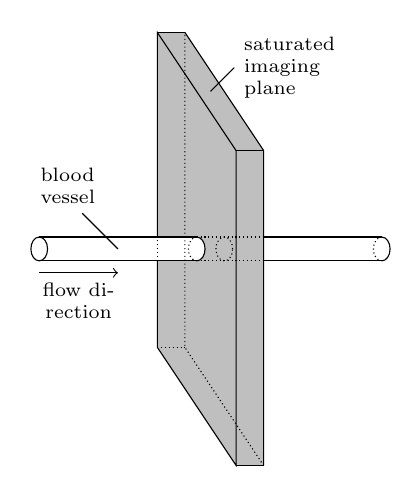
\begin{tikzpicture}
	\draw (2.85, 1ex) -- (4.35, 1ex);
	\draw (2.85, -1ex) -- (4.35, -1ex);
	\node (c) at (4.35, 0) {};
	\begin{scope}[shift={(c)}]
		\draw (0, -1ex) arc (-90:90:0.7ex and 1ex);
		\draw[densely dotted] (0, 1ex) arc (90:270:0.7ex and 1ex);
	\end{scope}

	\fill[lightgray] (1.5,  2.75) -- (1.85,  2.75) -- (2.85, 1.25) -- (2.85, -2.75) -- (2.5, -2.75) -- (1.5, -1.25) -- cycle;

	\fill[white] (0, -1ex) -- (2, -1ex) arc (-90:90:0.7ex and 1ex) -- (0, 1ex) arc (90:270:0.7ex and 1ex);

	\draw (0, 0) ellipse (0.7ex and 1ex);
	\node (a) at (2, 0) {};
	\begin{scope}[shift={(a)}]
		\draw (0, -1ex) arc (-90:90:0.7ex and 1ex);
		\draw[densely dotted] (0, 1ex) arc (90:270:0.7ex and 1ex);
	\end{scope}
	\draw[densely dotted] (2.35, 0) ellipse (0.7ex and 1ex);

	\draw (0, 1ex) -- (2, 1ex);
	\draw[densely dotted] (2, 1ex) -- (2.85, 1ex);

	\draw (0, -1ex) -- (2, -1ex);
	\draw[densely dotted] (2, -1ex) -- (2.85, -1ex);

	\draw (2.5, 1.25) -- (2.5, -2.75) -- (1.5, -1.25) -- (1.5, -1ex);
	\draw[densely dotted] (1.5, -1ex) -- (1.5, 1ex);
	\draw (1.5, 1ex) -- (1.5, 2.75) -- (2.5, 1.25);
	\draw (1.85, 2.75) -- (2.85, 1.25) -- (2.85, -2.75);
	\draw[densely dotted] (2.85, -2.75) -- (1.85, -1.25) -- (1.85, 2.75);
	\draw (2.5,  1.25) -- (2.85,  1.25);
	\draw (2.5, -2.75) -- (2.85, -2.75);
	\draw (1.5,  2.75) -- (1.85,  2.75);
	\draw[densely dotted] (1.5, -1.25) -- (1.85, -1.25);
	\draw (2.175, 2) -- ++ (2ex, 2ex) node [right, font=\scriptsize] {\parbox{10ex}{saturated imaging plane}};
	\draw (1, 0) -- ++ (-3ex, 3ex) node [above, font=\scriptsize] {\parbox{10ex}{blood \\ vessel}};
	\draw[->] (0, -2ex) -- node [below, font=\scriptsize] {\parbox{10ex}{\centering flow direction}} (1, -2ex);
\end{tikzpicture}